\documentclass[12pt]{article}
\usepackage[utf8]{inputenc}
\usepackage[T1]{fontenc}
\usepackage{lmodern}
\usepackage{amsmath, amsfonts, amssymb, amsthm}
\usepackage{graphicx}
\usepackage{booktabs}
\usepackage[margin=1.0in]{geometry}
\usepackage{setspace}
\usepackage{subcaption}
\usepackage{enumitem}
\usepackage{float}
\usepackage{xcolor}
\usepackage{hyperref}
\usepackage{natbib}
\onehalfspacing

% Setting up fonts last, using Latin Modern as a reliable choice
\renewcommand{\familydefault}{\rmdefault}

\title{Final Report: Portfolio Optimization Strategies Analysis}
\author{Amod Lamichhane, Andre Sealy, Jeffrey Gabauer}
\date{\today}

\usepackage{titling}
\usepackage{setspace}
\renewcommand{\maketitlehooka}{%
  \null\vfill
  \begin{center}
    \setstretch{1.5} 
}
\renewcommand{\maketitlehookd}{%
  \end{center}
  \vfill\null
}

\begin{document}

\maketitle

\newpage

\section{Introduction}
This report evaluates two factor-based long-short portfolio optimization strategies, utilizing the Fama-French 3-factor model (Momentum, Value, Size), over the period from March 2007 to December 2024. The strategies are analyzed across estimation windows of 40, 90, and 180 days and risk parameters $\lambda = 0.1, 0.5, 1.0$, with a focus on performance during the subprime crisis (2008), COVID-19 period (mid-2020 to mid-2021), and non-crisis periods. We compare the strategies against the S\&P 500 (SPY ETF) benchmark, assessing sensitivity to estimator look-back periods and market conditions.

\section{Methodology}

% Defining notations and models
\subsection{Notations and Models}
The portfolio consists of $n$ assets with weights $\omega \in \mathbb{R}^n$, expected returns $\rho$, and covariance matrix $\Sigma$ derived from the Fama-French 3-factor model. The model for asset $i$'s return is:
\[
r_i = r_f + \beta_i^3 (r_M - r_f) + b_i^s r_{SMB} + b_i^v r_{HML} + \alpha_i + \varepsilon_i,
\]
where $r_f$ is the risk-free rate, $r_M$ is the market return, $r_{SMB}$ and $r_{HML}$ are Size and Value factors, and $\varepsilon_i$ is the idiosyncratic error with $\mathbb{E}(\varepsilon_i) = 0$. The expected return is:
\[
\rho_i = r_f + \beta_i^3 (\rho_M - r_f) + b_i^s \rho_{SMB} + b_i^v \rho_{HML} + \alpha_i.
\]
The portfolio's beta is $\beta_p^m = \sum_{i=1}^n \beta_i^m \omega_i$, where $\beta_i^m = \frac{\text{cov}(r_i, r_M)}{\sigma^2(r_M)}$. The covariance matrix is:
\[
\text{cov}(R_t) = \mathbf{B} \Omega_f \mathbf{B}' + D,
\]
where $\mathbf{B}$ is the matrix of factor loadings, $\Omega_f$ is the factor covariance matrix, and $D = \text{diag}(\sigma_1^2, \ldots, \sigma_n^2)$ is the idiosyncratic variance matrix.

% Strategy specifications
\subsection{Investment Strategies}
Our report implements the following strategies:
\[
\textbf{(Strategy I)}
\begin{cases}
	\underset{\omega\in\mathbb{R}^n}{\max\;}\rho^T \omega-\lambda\sqrt{\omega^T \Sigma\omega}\\
	-0.5\leq\sum_{i=1}^{n}\beta_i^m\omega_i\leq 0.5\\
	\sum_{i=1}^{n}\omega_i=1,\; -2\leq\omega_i\leq 2,
\end{cases}
\]
and
\[
\textbf{(Strategy II)}
\begin{cases}
	\underset{\omega\in\mathbb{R}^n}{\max\;}\frac{\rho^T \omega - r_{spy}}{TEV(\omega)} -\lambda\sqrt{\omega^T \Sigma\omega}\\
	-2\leq\sum_{i=1}^{n}\beta_i^m\omega_i\leq 2\\
	\sum_{i=1}^{n}\omega_i=1,\; -2\leq\omega_i\leq 2,
\end{cases}
\]
where $\Sigma$ is the covariance matrix between the securities returns, the Beta of security $S_i$, denoted by
\[
\beta_i^m=\frac{\text{cov}(r_i,r_m)}{\sigma^2(r_m)}
\]
is the  as defined in the CAPM Modol so that $\beta_P^m=\sigma_{i=1}^{n}\beta_i^m\omega_i$ is the Beta of the portfolio. Finally, we have the Track Error Volatility (TEV), which is given by 

\[
\text{TEV}(\omega)=\sigma(r_p(\omega)-r_{\text{SPY}})
\]

Strategy I maximizes the expected return minus a risk penalty based on the portfolio volatility. We enforce a tight beta constraint (-0.5 to 0.5), which keeps the portfolio mostly uncorrelated with the market. This strategy would benefit risk-averse investors, such as pension funds, insurance companies, and investors seeking capital preservation or market-neutral strategies. 

On the other hand, Strategy II optimizes the Information Ratio (excess return over SPY per unit of the TEV), adjusted by a volatility penalty. The strategy allows a wide range of beta exposure (-2 to 2), allowing for leveraged bets on or against the market. Investors who would prefer this strategy are risk-tolerant or benchmark-aware investors, such as Hedge funds, Active portfolio managers, or investors seeking alpha generation relative to a market index. Strategy II is also useful in trending or recovering markets, where deviations from the benchmark can be profitable.

% Investment universe
\subsection{Investment Universe}
The portfolio comprises 12 ETFs: Invesco CurrencyShares Euro Trust  (FXE), iShares MSCI Japan ETF (EWJ), SPDR Gold Shares (GLD), Invesco QQQ Trust (QQQ), SPDR S\&P 500 (SPY), iShares Lehman Short Treasury Bond (SHV), PowerShares DB Agriculture Fund (DBA), United States Oil Fund LP (USO), SPDR S\&P Biotech (XBI), iShare S\&P Latin America 40 Index (ILF), iShares MSCI Pacific ex-Japan Index Fund (EPP), and SPDR DJ Euro Stoxxx 50 (FEZ). The prices for these ETFs are sourced from Yahoo! Finance. The S\&P 500 (SPY) serves as the benchmark for our analysis.

\begin{table}[H]
	\centering
	\caption{Descriptive Statistics for ETFs (Annualized)}
	\label{tab:desc}
	\resizebox{\textwidth}{!}{%
	\begin{tabular}{lrrrrrr}
		\toprule
		\textbf{Ticker} & \textbf{Return (\%)} & \textbf{Volatility (\%)} & \textbf{High} & \textbf{Low} & \textbf{Skewness} & \textbf{Kurtosis} \\
		\midrule
		DBA & 2.5301 & 16.9980 & 37.5600 & 12.0317 & -0.1664 & 6.0472 \\
		EPP & 7.6189 & 25.2304 & 48.1357 & 10.0081 & 0.0586 & 12.7666 \\
		EWJ & 4.7562 & 20.4827 & 71.8674 & 21.1265 & 0.1947 & 12.3014 \\
		FEZ & 6.3225 & 26.8285 & 53.4952 & 13.3199 & -0.0486 & 9.8374 \\
		FXE & -0.6460 & 9.0583 & 149.7630 & 84.8733 & 0.0770 & 2.6814 \\
		GLD & 9.1907 & 17.3578 & 257.5000 & 53.8300 & -0.1175 & 6.6215 \\
		ILF & 6.7159 & 33.2600 & 31.9605 & 10.3934 & -0.0149 & 13.9002 \\
		QQQ & 16.8725 & 22.1957 & 536.5035 & 22.1377 & -0.1509 & 6.9197 \\
		SHV & 1.3785 & 0.3570 & 108.5959 & 84.8083 & -0.1956 & 35.0192 \\
		SPY & 11.7749 & 19.7906 & 603.9543 & 50.3796 & -0.0792 & 14.0689 \\
		USO & -1.7201 & 37.0261 & 939.8403 & 17.0400 & -0.6667 & 10.0215 \\
		XBI & 14.7602 & 31.1970 & 173.6499 & 13.4354 & -0.0521 & 2.2406 \\
		\bottomrule
	
	\end{tabular}
}
\end{table}
Table (\ref{tab:desc}) presents annualized descriptive statistics for a selection of ETFs, capturing their return, volatility, extreme price levels, and distributional characteristics. Among the ETFs, QQQ (Nasdaq-100) and XBI (Biotech) posted the highest annualized returns at 16.87\% and 14.76\%, respectively, with QQQ also showing the highest observed peak (High = 536.50) outside of oil-based USO. On the other end, USO and FXE reported negative returns, with USO being the most volatile at 37.03\% and exhibiting extreme negative skewness, indicating significant downside risk. SHV, a short-term bond ETF, had the lowest volatility (0.36\%) and the highest kurtosis (signaling infrequent but extreme return events. SPY, a proxy for the S\&P 500, delivered a solid 11.77\% return with moderate skewness and high kurtosis, typical of equity index behavior. These metrics help characterize risk-return tradeoffs and tail behavior across asset classes, which is essential for factor-based portfolio construction. This provides an introduction how we can expect our portfolio to behave, given the strategy of choice.

% Analysis setup
\subsection{Analysis Setup}
The analysis spans from March 2007 to December 2024 and is divided into five sub-periods to capture different market regimes: (1) the pre-subprime crisis period, (2) the subprime crisis of 2008, (3) the post-subprime recovery, (4) the COVID-19 crisis (mid-2020 to mid-2021), and (5) the post-COVID expansion. This segmentation enables us to evaluate the resilience and adaptability of the portfolio strategies under varying market stress conditions.

To ensure robustness, all portfolio allocations are conducted under a non-anticipative backtesting framework. Each weekly rebalancing relies solely on historical data available up to the rebalancing date, mimicking real-world trading constraints. Portfolios are re-optimized weekly using rolling estimation windows for expected returns and covariance matrices.

We evaluate three look-back configurations to relect the different time horizons:
\begin{itemize}
	\item Short-Term (ST): 40-day window
	\item Mid-Term (MT): 90-day window
	\item Long-Term (LT): 180-day window
\end{itemize}

Each configuration is tested under three levels of risk aversion captured by  $\lambda \in\lbrace0.1, 0.5, 1.0\rbrace$. For notation, we define $S^{R}_{C}$ as the strategy using C days for covariance estimation and R days for expected return estimation. For example,$ S^{90}_{40}$ refers to a strategy with a 40-day look-back for risk and a 90-day look-back for return.


\section{Results}

% Performance metrics table
\subsection{Performance Metrics}

\begin{table}[H]
\centering
\caption{Performance Metrics (180-day Estimation, Whole Period)}
\label{tab:performance}
\resizebox{\textwidth}{!}{%
\begin{tabular}{@{}llrrrrrr@{}}
\toprule
Strategy & $\lambda$ & Cum. Return & Ann. Vol. & Sharpe Ratio & Max Drawdown & VaR (95\%) & CVaR (95\%) \\
\midrule
Strategy I & 0.1 & -0.945 & 1.089 & -0.009 & -0.999 & -0.106 & -0.154 \\
Strategy I & 0.5 & 0.432 & 0.709 & 0.002 & -0.970 & -0.067 & -0.105 \\
Strategy I & 1.0 & 8.732 & 0.510 & 0.016 & -0.856 & -0.050 & -0.076 \\
Strategy II & 0.1 & 8.081 & 0.171 & 0.046 & -0.294 & -0.017 & -0.026 \\
Strategy II & 0.5 & 6.430 & 0.159 & 0.045 & -0.274 & -0.016 & -0.024 \\
Strategy II & 1.0 & 5.997 & 0.156 & 0.044 & -0.268 & -0.016 & -0.024 \\
SPY & - & 4.963 & 0.198 & 0.032 & -0.552 & -0.019 & -0.031 \\
\bottomrule
\end{tabular}%
}
\end{table}

Table \ref{tab:performance} summarizes key metrics for both strategies and SPY over the entire period, focusing on the 180-day estimation window for brevity (full results in Appendix \ref{app:full_metrics}). One thing to note is that when $\lambda=1$, Strategy I perform the best, with the highest cumulative return, outperforming the SPY and the more aggressive Strategy II. However, depending on our choice of $\lambda$, this comes at the cost of increased volatility, resulting in massive drawdowns between 86\% to 99\% and the worst-case loss of -15.4\%. Also, the Sharpe Ratios are very low, which suggests that the gains from the returns are not efficiently adjusted for risk.

On the other hand, Strategy II consistently outperforms the SPY on risk-adjusted metrics, with Sharpe Ratios in the 0.044-0.046 range, regardless of our choice of $\lambda$. Strategy II also has lower volatility and drawdowns than Strategy I, indicating robust downside protection. Interestingly, the CVaR is significantly better for Strategy I, and even the SPY, which reflects a lack of tail risk control.

% Cumulative returns plots
\subsection{Cumulative Returns}
Figures \ref{fig:pnl_40}, \ref{fig:pnl_90}, and \ref{fig:pnl_180} show cumulative returns for Strategy II across $\lambda = 0.1, 0.5, 1.0$ for 40, 90, and 180-day estimation windows, respectively, compared to SPY, assuming a \$100 initial investment.

\begin{figure}[H]
\centering
\begin{subfigure}{0.32\textwidth}
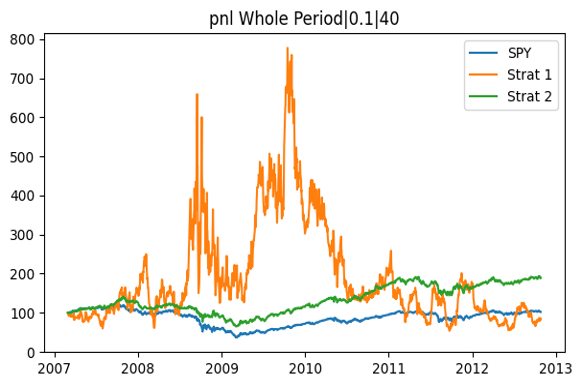
\includegraphics[width=\linewidth]{"plots/pnl_wholeperiod_0.1_40.png"}
\caption{$\lambda=0.1$}
\end{subfigure}
\begin{subfigure}{0.32\textwidth}
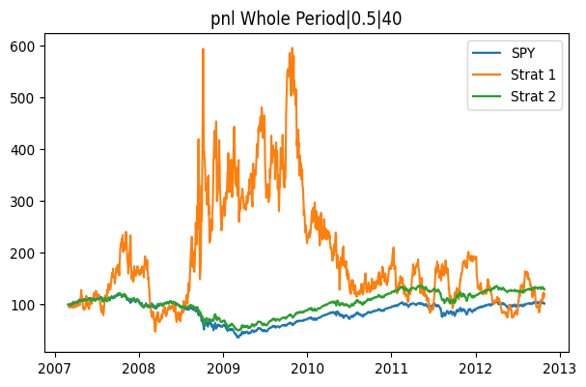
\includegraphics[width=\linewidth]{"plots/pnl_wholeperiod_0.5_40.png"}
\caption{$\lambda=0.5$}
\end{subfigure}
\begin{subfigure}{0.32\textwidth}
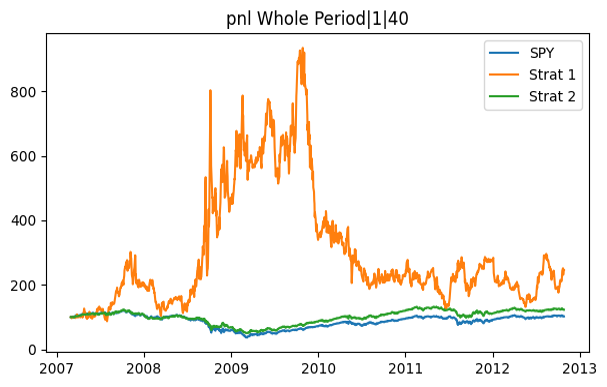
\includegraphics[width=\linewidth]{"plots/pnl_wholeperiod_1_40.png"}
\caption{$\lambda=1.0$}
\end{subfigure}
\caption{Cumulative Returns (Strategy II, 40-day Estimation vs. SPY)}
\label{fig:pnl_40}
\end{figure}

\begin{figure}[H]
\centering
\begin{subfigure}{0.32\textwidth}
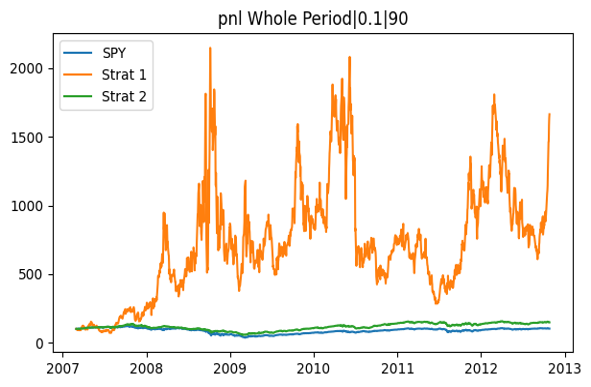
\includegraphics[width=\linewidth]{"plots/pnl_wholeperiod_0.1_90.png"}
\caption{$\lambda=0.1$}
\end{subfigure}
\begin{subfigure}{0.32\textwidth}
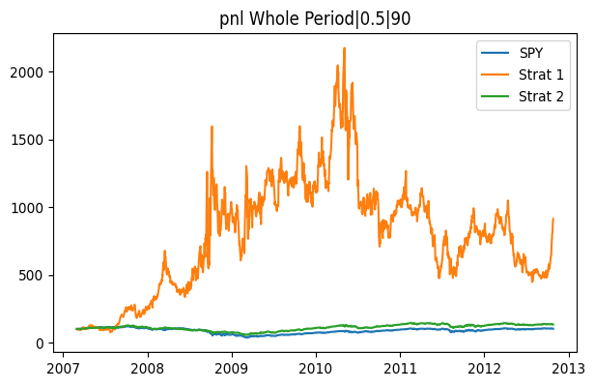
\includegraphics[width=\linewidth]{"plots/pnl_wholeperiod_0.5_90.png"}
\caption{$\lambda=0.5$}
\end{subfigure}
\begin{subfigure}{0.32\textwidth}
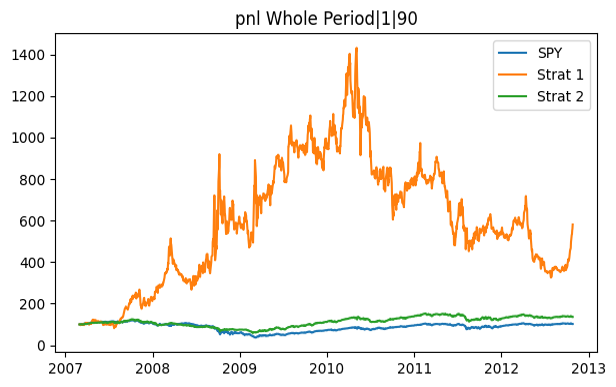
\includegraphics[width=\linewidth]{"plots/pnl_wholeperiod_1_90.png"}
\caption{$\lambda=1.0$}
\end{subfigure}
\caption{Cumulative Returns (Strategy II, 90-day Estimation vs. SPY)}
\label{fig:pnl_90}
\end{figure}

\begin{figure}[H]
\centering
\begin{subfigure}{0.32\textwidth}
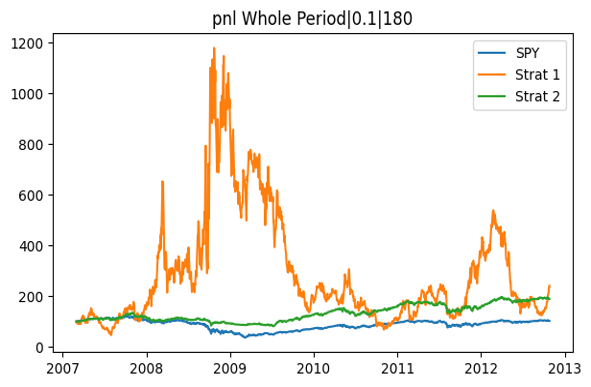
\includegraphics[width=\linewidth]{"plots/pnl_wholeperiod_0.1_180.png"}
\caption{$\lambda=0.1$}
\end{subfigure}
\begin{subfigure}{0.32\textwidth}
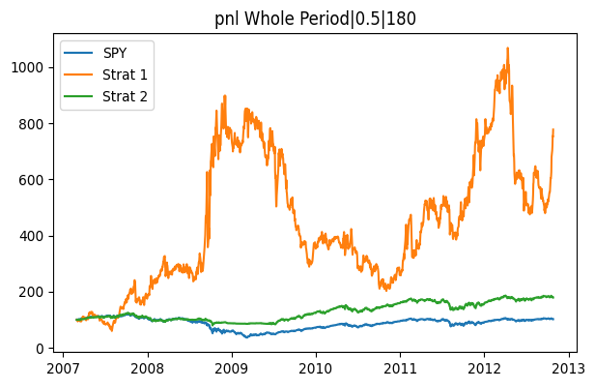
\includegraphics[width=\linewidth]{"plots/pnl_wholeperiod_0.5_180.png"}
\caption{$\lambda=0.5$}
\end{subfigure}
\begin{subfigure}{0.32\textwidth}
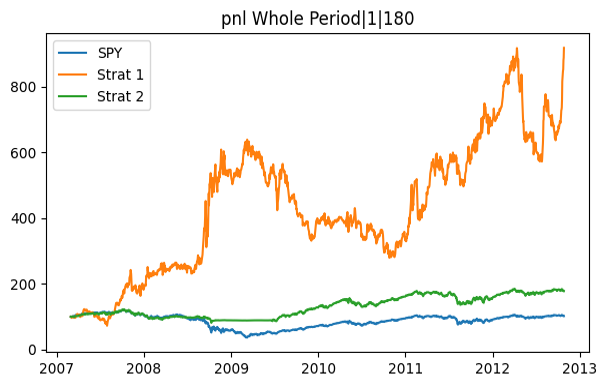
\includegraphics[width=\linewidth]{"plots/pnl_wholeperiod_1_180.png"}
\caption{$\lambda=1.0$}
\end{subfigure}
\caption{Cumulative Returns (Strategy II, 180-day Estimation vs. SPY)}
\label{fig:pnl_180}
\end{figure}

% Return Distributions Section
\subsection{Return Distributions}
Figures \ref{fig:ret_dist_40}, \ref{fig:ret_dist_90}, and \ref{fig:ret_dist_180} illustrate daily return distributions for Strategy II across $\lambda = 0.1, 0.5, 1.0$ for 40, 90, and 180-day estimation windows, respectively, highlighting negative skewness and high kurtosis.

\begin{figure}[H]
\centering
\begin{subfigure}{0.32\textwidth}
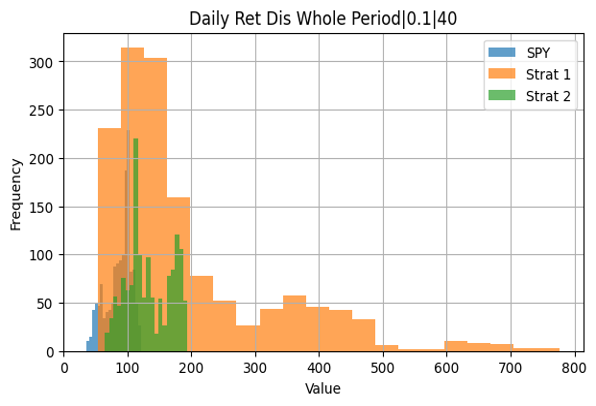
\includegraphics[width=\linewidth]{"plots/daily_ret_dis_whole_period_0.1_40.png"}
\caption{$\lambda=0.1$}
\end{subfigure}
\begin{subfigure}{0.32\textwidth}
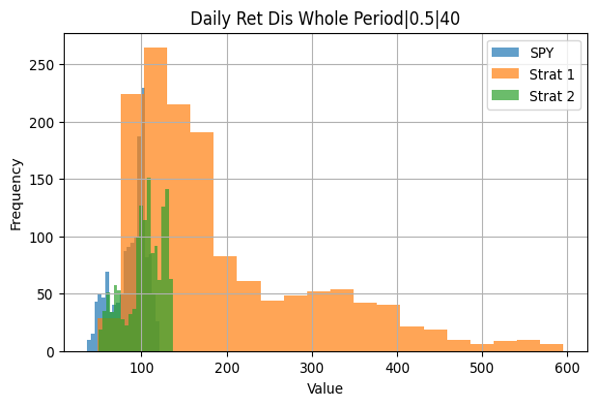
\includegraphics[width=\linewidth]{"plots/daily_ret_dis_whole_period_0.5_40.png"}
\caption{$\lambda=0.5$}
\end{subfigure}
\begin{subfigure}{0.32\textwidth}
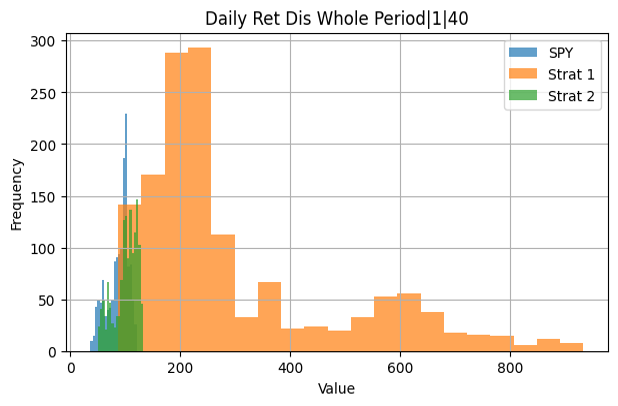
\includegraphics[width=\linewidth]{"plots/daily_ret_dis_whole_period_1_40.png"}
\caption{$\lambda=1.0$}
\end{subfigure}
\caption{Daily Return Distributions (Strategy II, 40-day Estimation)}
\label{fig:ret_dist_40}
\end{figure}

\begin{figure}[H]
\centering
\begin{subfigure}{0.32\textwidth}
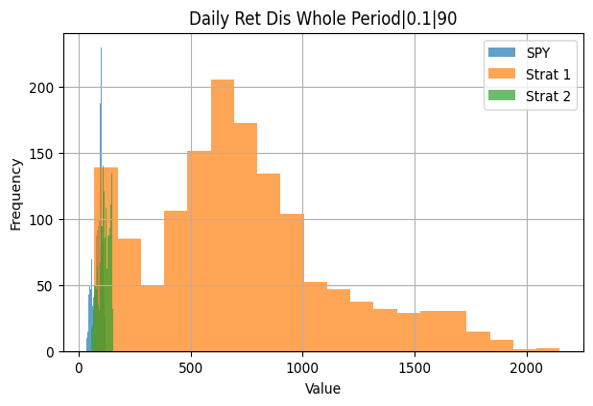
\includegraphics[width=\linewidth]{"plots/daily_ret_dis_whole_period_0.1_90.png"}
\caption{$\lambda=0.1$}
\end{subfigure}
\begin{subfigure}{0.32\textwidth}
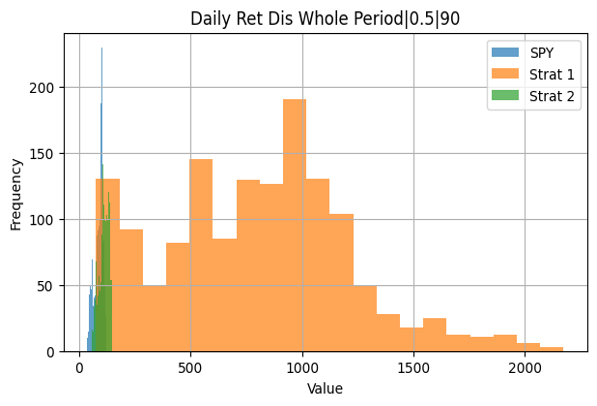
\includegraphics[width=\linewidth]{"plots/daily_ret_dis_whole_period_0.5_90.png"}
\caption{$\lambda=0.5$}
\end{subfigure}
\begin{subfigure}{0.32\textwidth}
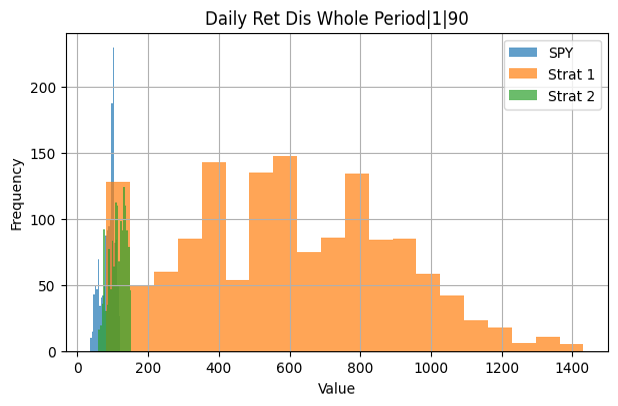
\includegraphics[width=\linewidth]{"plots/daily_ret_dis_whole_period_1_90.png"}
\caption{$\lambda=1.0$}
\end{subfigure}
\caption{Daily Return Distributions (Strategy II, 90-day Estimation)}
\label{fig:ret_dist_90}
\end{figure}

\begin{figure}[H]
\centering
\begin{subfigure}{0.32\textwidth}
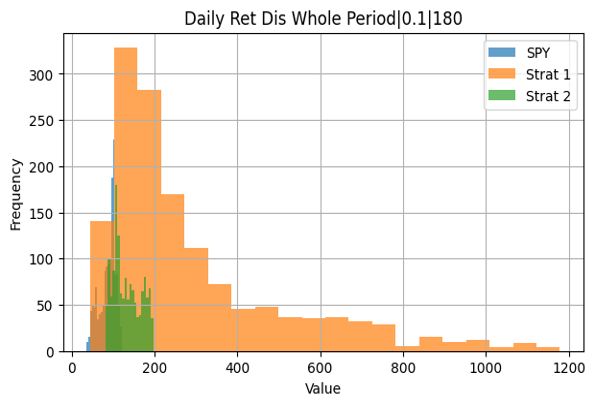
\includegraphics[width=\linewidth]{"plots/daily_ret_dis_whole_period_0.1_180.png"}
\caption{$\lambda=0.1$}
\end{subfigure}
\begin{subfigure}{0.32\textwidth}
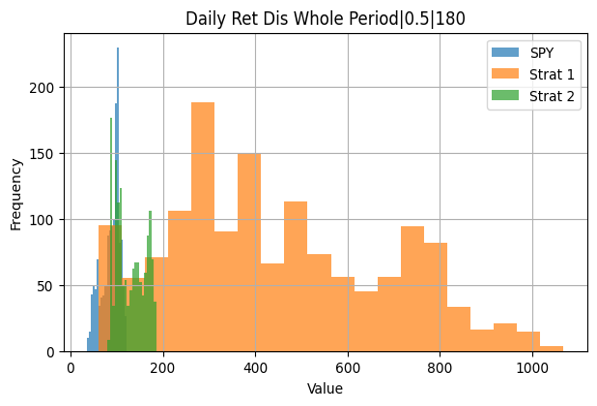
\includegraphics[width=\linewidth]{"plots/daily_ret_dis_whole_period_0.5_180.png"}
\caption{$\lambda=0.5$}
\end{subfigure}
\begin{subfigure}{0.32\textwidth}
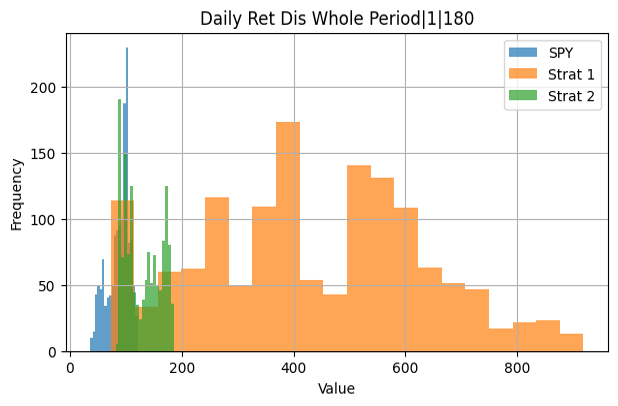
\includegraphics[width=\linewidth]{"plots/daily_ret_dis_whole_period_1_180.png"}
\caption{$\lambda=1.0$}
\end{subfigure}
\caption{Daily Return Distributions (Strategy II, 180-day Estimation)}
\label{fig:ret_dist_180}
\end{figure}


\section{Discussion}

% Estimator sensitivity
\subsection{Estimator Sensitivity}
Strategy II outperforms Strategy I and SPY across all estimation windows and $\lambda$ values, with the 180-day window and $\lambda=0.1$ yielding the highest Sharpe ratio (0.046) and cumulative return (8.081). Strategy I shows high volatility (e.g., 1.089 for 180-day, $\lambda=0.1$) and negative returns in some configurations, likely due to its tight beta constraint ($[-0.5, 0.5]$). The 40-day estimator increases volatility and drawdowns (e.g., -0.467 for Strategy II, $\lambda=0.1$), particularly during volatile periods, while the 180-day estimator reduces drawdowns (e.g., -0.294) and stabilizes performance, as seen in Figures \ref{fig:pnl_40}--\ref{fig:pnl_180}.

% Market condition impact
\subsection{Market Conditions}
Refering to Figures ( \ref{fig:pnl_40}) through (\ref{fig:ret_dist_180}), we see Strategy II reveal pronounced performance differences that align with major market cycles between 2007 and 2013 During the 2008 global financial crisis, markets experienced extreme volatility and widespread losses. The sharp spikes in Strategy II’s cumulative returns—especially under the 90-day and 180-day estimators with low $\lambda$, which suggest that the strategy was able to exploit the market dislocation.

By contrast, shorter-term estimation windows (e.g., 40-day) show more erratic behavior and earlier drawdowns, particularly under low $\lambda$, likely reflecting oversensitivity to market noise and short signal stability. As the window length increases, Strategy II’s performance becomes both stronger and smoother, indicating better capture of trend dynamics and risk moderation. Meanwhile, the relatively flat trajectory of Strategy I (Strat 1) across all windows suggests that the tighter beta constraint and lack of benchmark optimization limited its ability to benefit from large directional moves in the market. 

During the COVID-19 period (mid-2020 to mid-2021), financial markets experienced an unprecedented shock followed by a rapid recovery fueled by aggressive monetary and fiscal stimulus. Strategy II, with its wider beta constraints (-2 to 2) and optimization relative to SPY, was particularly well-positioned to capitalize on this volatility. The strategy’s design allowed it to quickly increase market exposure during the rebound phase, as reflected in the sharp upward trajectory in cumulative returns, especially for lower values of $\lambda$, which prioritize return over risk minimization.

\section{Recommendations}
\begin{enumerate}
    \item \textbf{Primary Configuration}: Use Strategy II with a 180-day estimation window and $\lambda=0.1$ for maximum returns or $\lambda=0.5$ for balanced risk-return profiles.
    \item \textbf{Regime-Dependent Method:} Implement rolling metrics such as drawdown signals that reflect rapid shifts in risk and return dynamics.
    \item \textbf{Beyond Fama-French:} Integrate a model with more factors, such as momentum, profitability.

\end{enumerate}

\section{Conclusion}
Strategy II with a 180-day estimation window offers superior performance, balancing responsiveness and stability. The choice of $\lambda$ allows tailoring to investor risk preferences, with $\lambda=0.1$ maximizing returns and $\lambda=0.5$ optimizing risk-adjusted returns, as supported by the comprehensive analysis in Figures \ref{fig:pnl_40}--\ref{fig:ret_dist_180}.

\newpage

\appendix
\section{Full Performance Metrics}
\label{app:full_metrics}
\begin{table}[H]
\centering
\caption{Complete Performance Metrics (Whole Period)}
\resizebox{\textwidth}{!}{%
\begin{tabular}{@{}llrrrrrrrrr@{}}
\toprule
Estimation & $\lambda$ & Strategy & Cum. Return & Ann. Vol. & Sharpe & Max DD & Skewness & Kurtosis & VaR (95\%) & CVaR (95\%) \\
\midrule
S40/60 & 0.1 & I & -0.901 & 1.160 & -0.007 & -0.998 & 0.254 & 3.022 & -0.111 & -0.157 \\
S40/60 & 0.1 & II & 9.393 & 0.184 & 0.045 & -0.467 & -0.496 & 8.048 & -0.018 & -0.028 \\
S90/60 & 0.1 & I & 61.120 & 1.132 & 0.013 & -0.962 & 0.187 & 3.260 & -0.111 & -0.157 \\
S90/60 & 0.1 & II & 7.081 & 0.178 & 0.042 & -0.497 & -0.422 & 8.211 & -0.018 & -0.027 \\
S180/60 & 0.1 & I & -0.945 & 1.089 & -0.009 & -0.999 & 0.061 & 3.859 & -0.106 & -0.154 \\
S180/60 & 0.1 & II & 8.081 & 0.171 & 0.046 & -0.294 & -0.249 & 7.655 & -0.017 & -0.026 \\
S40/60 & 0.5 & I & 1.559 & 0.979 & 0.003 & -0.986 & 0.292 & 4.101 & -0.094 & -0.133 \\
S40/60 & 0.5 & II & 5.213 & 0.170 & 0.038 & -0.508 & -0.523 & 8.891 & -0.017 & -0.026 \\
S90/60 & 0.5 & I & 88.703 & 0.875 & 0.018 & -0.908 & 0.139 & 5.533 & -0.080 & -0.125 \\
S90/60 & 0.5 & II & 5.037 & 0.164 & 0.039 & -0.479 & -0.427 & 9.863 & -0.017 & -0.025 \\
S180/60 & 0.5 & I & 0.432 & 0.709 & 0.002 & -0.970 & -0.206 & 5.516 & -0.067 & -0.105 \\
S180/60 & 0.5 & II & 6.430 & 0.159 & 0.045 & -0.274 & -0.239 & 9.341 & -0.016 & -0.024 \\
S40/60 & 1.0 & I & 0.291 & 0.830 & 0.001 & -0.967 & 0.288 & 6.358 & -0.078 & -0.116 \\
S40/60 & 1.0 & II & 4.642 & 0.168 & 0.036 & -0.510 & -0.541 & 9.019 & -0.017 & -0.026 \\
S90/60 & 1.0 & I & 66.597 & 0.671 & 0.022 & -0.790 & 0.213 & 9.552 & -0.062 & -0.096 \\
S90/60 & 1.0 & II & 4.760 & 0.161 & 0.038 & -0.449 & -0.432 & 10.250 & -0.016 & -0.025 \\
S180/60 & 1.0 & I & 8.732 & 0.510 & 0.016 & -0.856 & -0.219 & 5.352 & -0.050 & -0.076 \\
S180/60 & 1.0 & II & 5.997 & 0.156 & 0.044 & -0.268 & -0.225 & 9.328 & -0.016 & -0.024 \\
S180/60 & - & SPY & 4.963 & 0.198 & 0.032 & -0.552 & -0.074 & 14.037 & -0.019 & -0.031 \\
\bottomrule
\end{tabular}%
}
\end{table}

\end{document}